\chapter{状态机建模}

\section{从进程模板打开状态机}
在进程模板的类图上右键,呼出右键菜单,点击[编辑状态机],即可打开对应的状态机的编辑面板,如图\ref{statemachine_panel}所示。
\begin{figure}[h]
	\centering
	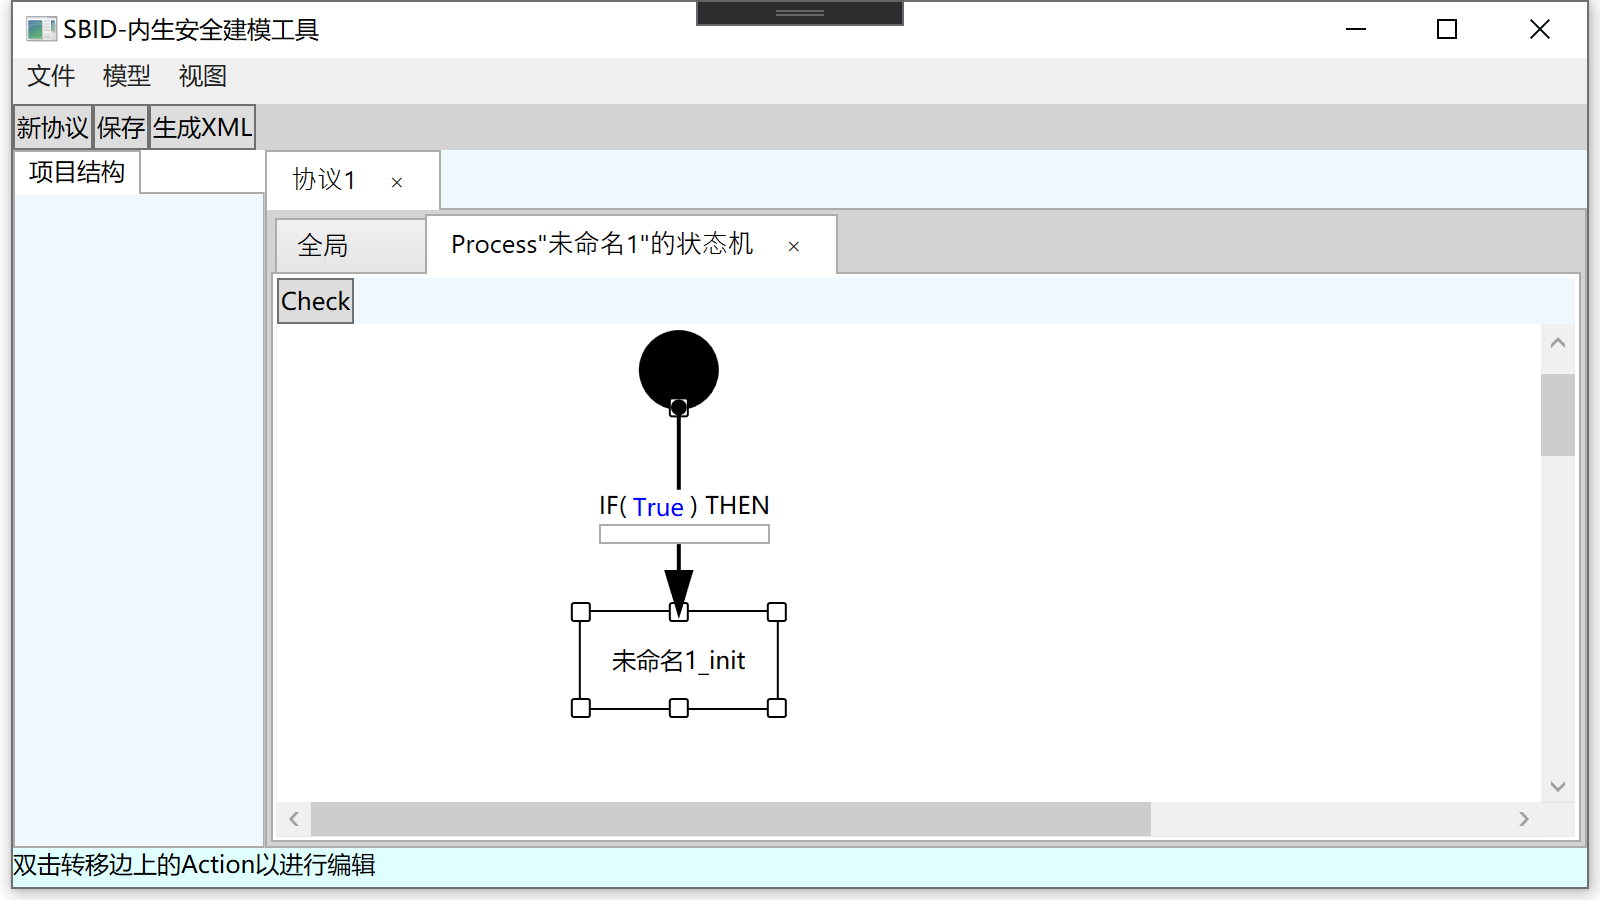
\includegraphics[width=12cm,height=6.75cm]{imgs/statemachine_panel.png}
	\caption{编辑状态机}
	\label{statemachine_panel}
\end{figure}
\par
可以看到,默认情况下,为进程模板的状态机创建了一个初始状态,及一个无条件到达的状态。
\par
在sbid中,每个进程模板对应一个唯一的状态机,状态机可以嵌套定义在多个面板中*。状态机转移边上的第一排文字表示转移边上的Guard条件,下方的列表指定边上的若干Action。

\section{编辑状态机}
在状态机面板上可对状态机进行编辑。
\subsection{状态机结构的修改}
在状态机面板空白处右键,在呼出的右键菜单中可以选择[创建普通状态结点]和[创建终止状态结点]的操作,在面板上的状态机结点的锚点上按住拖动,拖拽到另一状态的锚点上即可完成状态机的连线,如图\ref{statemachine_edit_structure}所示。
\begin{figure}[h]
	\centering
	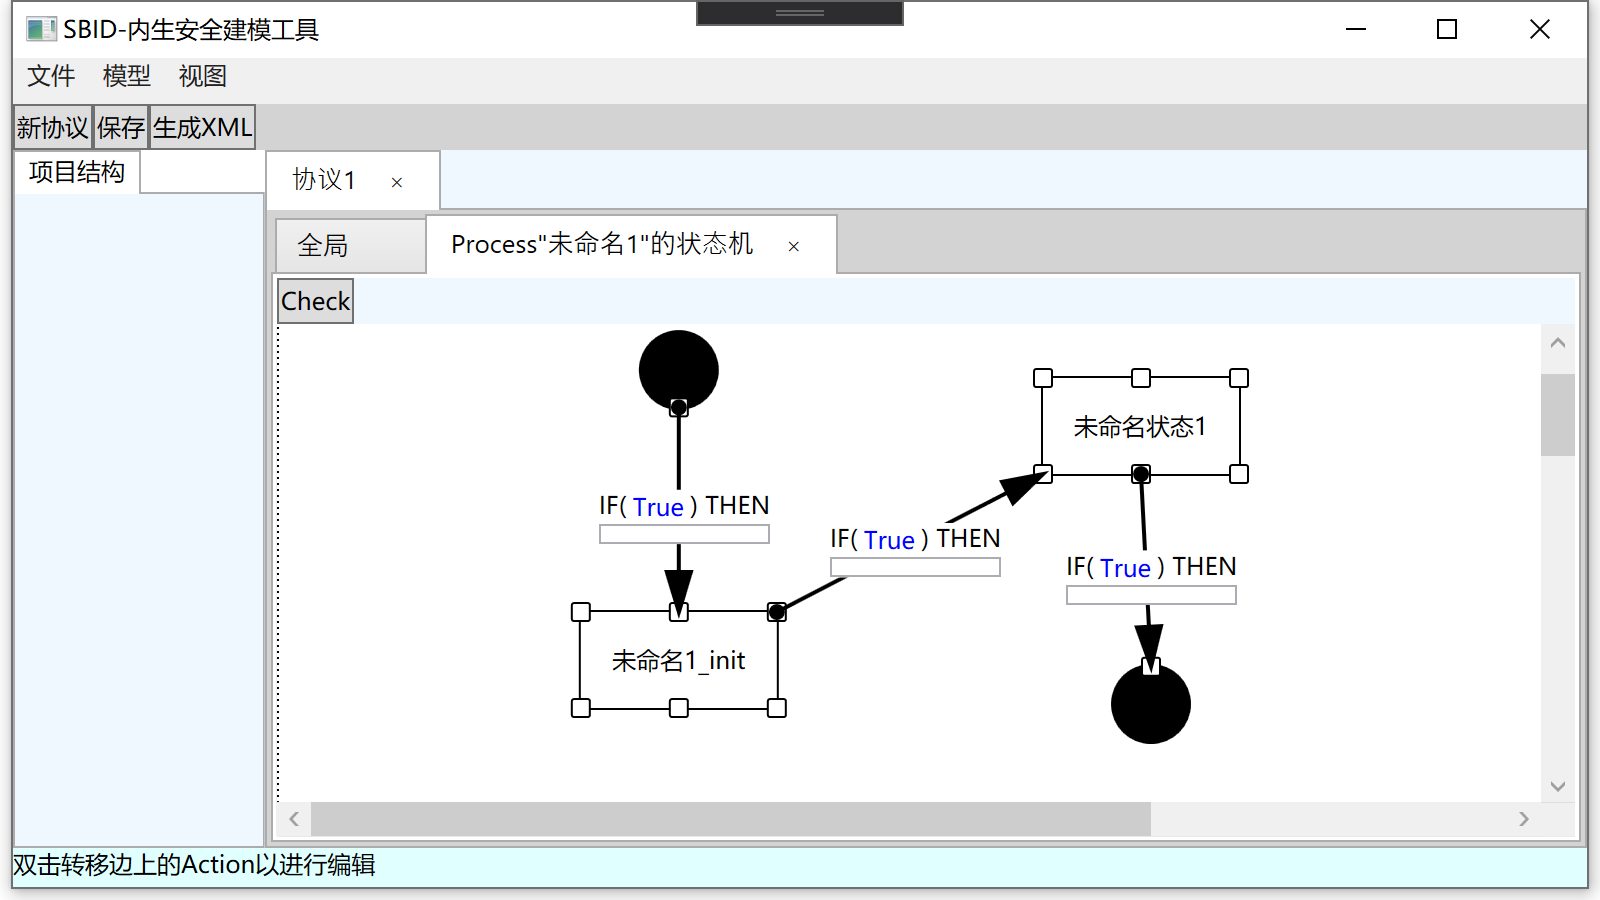
\includegraphics[width=12cm,height=6.75cm]{imgs/statemachine_edit_structure.png}
	\caption{添加了新结点并连线后的状态机}
	\label{statemachine_edit_structure}
\end{figure}
\subsection{状态机的状态和转移边的修改}
在状态机的状态上可以直接编辑其状态名称;在状态机的转移边上可以直接编辑Guard条件;双击转移边上的Action列表块,将会呼出修改Action的对话框,可以添加若干条要执行的Aciton,如图\ref{statemachine_edit_action}所示。
\begin{figure}[h]
	\centering
	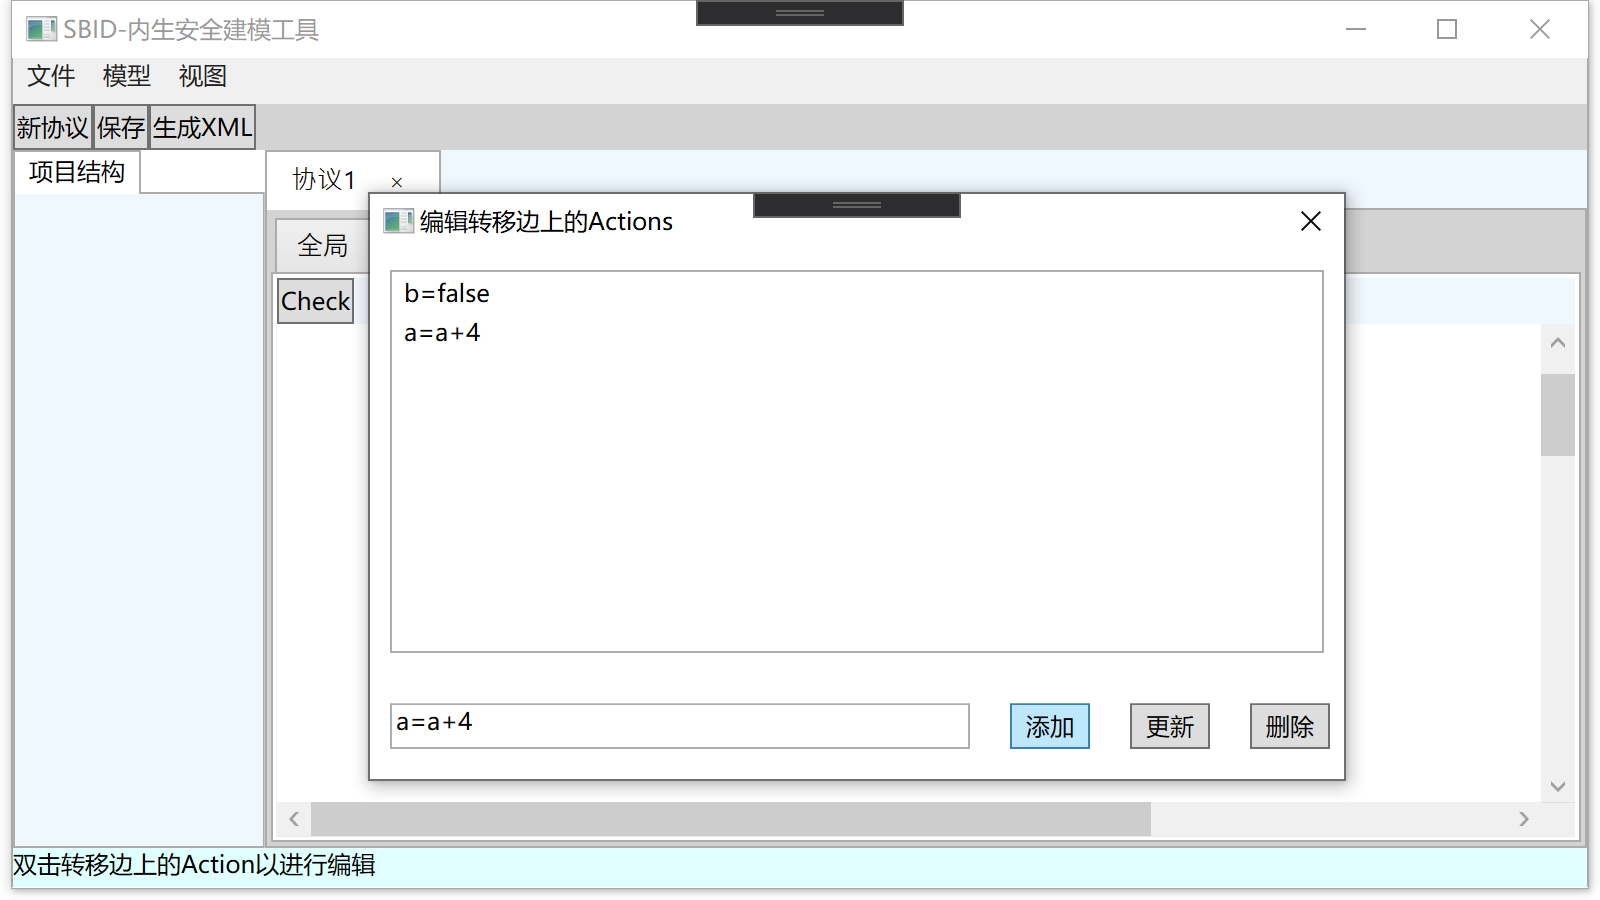
\includegraphics[width=12cm,height=6.75cm]{imgs/statemachine_edit_action.png}
	\caption{编辑状态机的转移边}
	\label{statemachine_edit_action}
\end{figure}
\par
修改Guard条件和Action后的状态机,如图\ref{statemachine_edited_action}所示。
\begin{figure}[h]
	\centering
	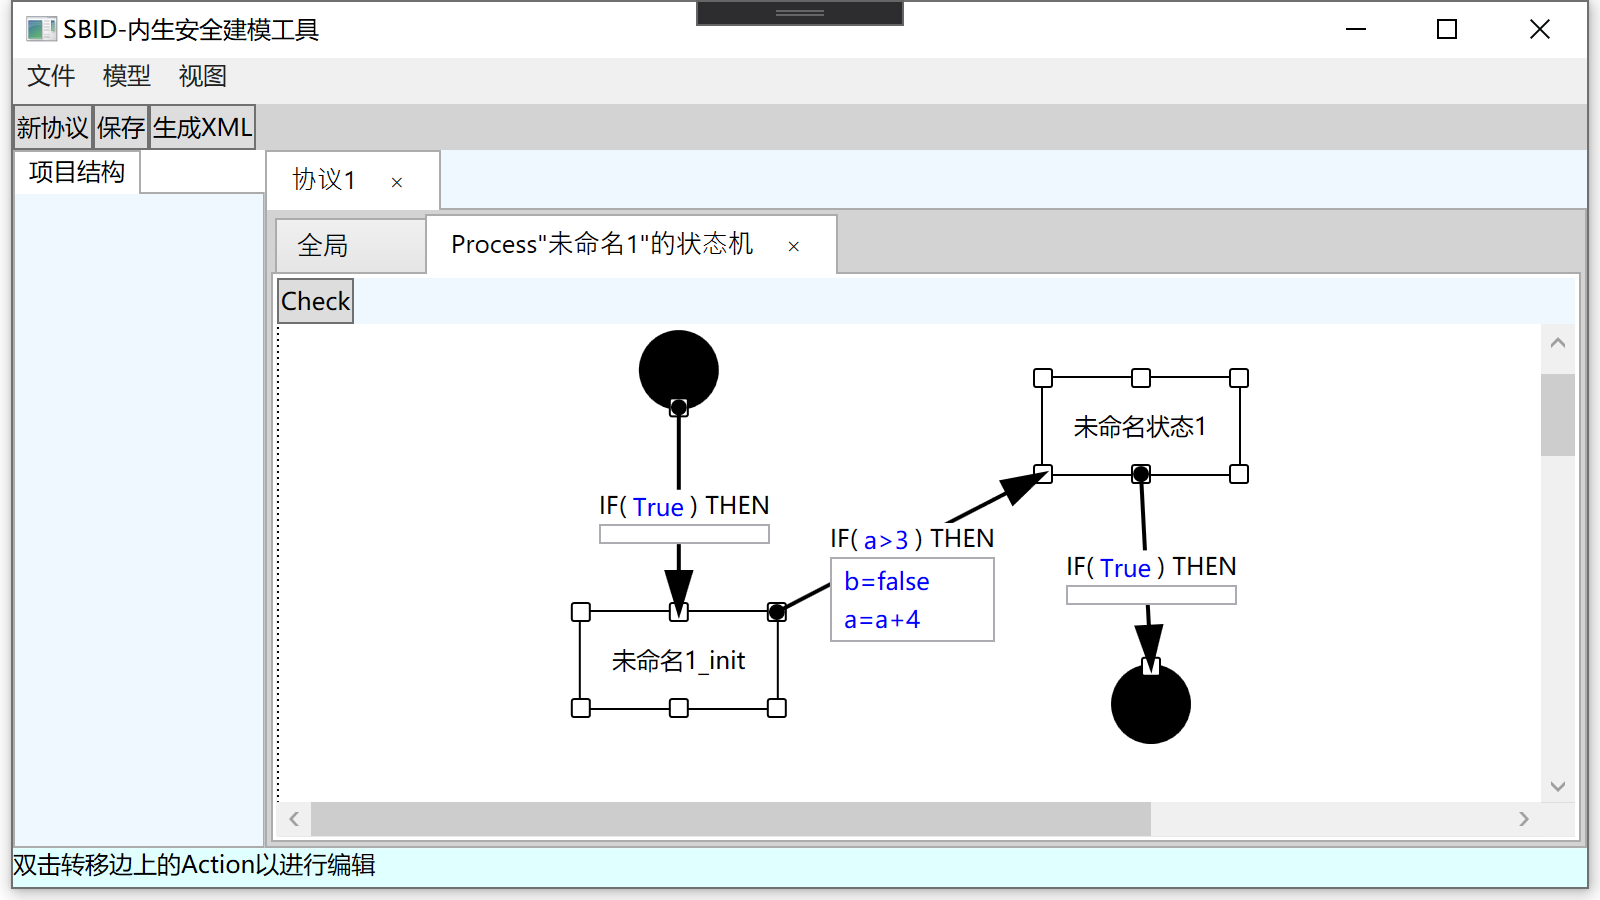
\includegraphics[width=12cm,height=6.75cm]{imgs/statemachine_edited_action.png}
	\caption{修改后的状态机}
	\label{statemachine_edited_action}
\end{figure}

\section{状态机嵌套}
未开发
